\documentclass[sigplan,10pt]{acmart}
\usepackage[utf8]{inputenc}

\setcopyright{rightsretained}
\copyrightyear{2020}
\acmYear{2020}
\acmDOI{}
\acmConference[]{}{}{}
\acmBooktitle{}
\acmPrice{}
\acmISBN{}

\begin{document}
\title{PushPin: Towards Production-Quality  Peer-to-Peer Collaboration}

\author{Peter van Hardenberg}
\email{pvh@inkandswitch.com}
\affiliation{%
  \institution{Ink \& Switch, LLC}
  \city{San Francisco}
  \state{CA}
  \postcode{}
  \country{USA}
}

\author{Martin Kleppmann}
\email{mk428@cl.cam.ac.uk}
\orcid{0000-0001-7252-6958}
\affiliation{%
  \institution{University of Cambridge}
  \streetaddress{15 JJ Thomson Avenue}
  \city{Cambridge}
  \state{}
  \postcode{CB3 0FD}
  \country{United Kingdom}
}

\begin{abstract}
Fully peer-to-peer application software promises many benefits over cloud software, in particular, being able to function indefinitely without requiring servers.
Research on distributed consistency mechanisms such as CRDTs has laid the foundation for P2P data synchronisation and collaboration.
In this paper we report on our experience in taking these technologies beyond research prototypes, and working towards commercial-grade P2P collaboration software.
We identify approaches that work well in our experience, such as the functional reactive programming paradigm, and highlight areas in need of further research, such as the reliability of NAT traversal and usability challenges.
\end{abstract}

\begin{CCSXML}
<ccs2012>
    <concept>
        <concept_id>10003033.10003039.10003051.10003052</concept_id>
        <concept_desc>Networks~Peer-to-peer protocols</concept_desc>
        <concept_significance>500</concept_significance>
    </concept>
    <concept>
        <concept_id>10011007.10010940.10010971.10010972.10010540</concept_id>
        <concept_desc>Software and its engineering~Peer-to-peer architectures</concept_desc>
        <concept_significance>500</concept_significance>
    </concept>
    <concept>
        <concept_id>10003120.10003130.10003233</concept_id>
        <concept_desc>Human-centered computing~Collaborative and social computing systems and tools</concept_desc>
        <concept_significance>500</concept_significance>
    </concept>
    <concept>
        <concept_id>10011007.10010940.10010992.10010993.10010961</concept_id>
        <concept_desc>Software and its engineering~Synchronization</concept_desc>
        <concept_significance>300</concept_significance>
    </concept>
</ccs2012>
\end{CCSXML}

\ccsdesc[500]{Networks~Peer-to-peer protocols}
\ccsdesc[500]{Software and its engineering~Peer-to-peer architectures}
\ccsdesc[500]{Human-centered computing~Collaborative and social computing systems and tools}
\ccsdesc[300]{Software and its engineering~Synchronization}

\keywords{real-time collaboration, CRDTs, peer-to-peer protocols, distributed programming, usability}

\maketitle

\section{Introduction}

In the past, software used to run on one computer and store its data on the local disk.
Now, increasingly, we expect our software and data to be available on multiple devices, enabling both synchronisation across devices belonging to the same user (e.g.\ laptop, smartphone, tablet), and allowing real-time collaboration between multiple users.

The standard way of implementing such multi-user, multi-device software today is to rely on cloud services that store the primary copy of the users' data, and which can be accessed through thin clients such as web browsers and mobile apps.
However, reliance on the cloud comes with problems: services require ongoing maintenance by expensive 24/7 operations teams, and they cease to exist when the organisation backing them terminates their funding.
If a cloud service shuts down, users lose access to all data stored in that service, unless some migration path to an alternative service is provided.
Moreover, cloud-centric software often does not work well offline, and can be slow as the client waits for round-trips to the server in order to load or store data there.

Peer-to-peer application software promises to overcome these problems.
In principle, a P2P system should be able to function indefinitely, without depending on someone paying the server bills to keep a cloud service running.
Storing the primary copy of data on the users' devices enables offline work and stronger data ownership~\cite{LocalFirst}, and synchronising updates through a P2P network should allow the same kind of real-time collaboration that we know from cloud software.

% maybe rather than "without relying on servers" we should say something like "servers are optional, software continues working even without servers"

While various research prototypes of P2P collaboration software have been developed, we are yet to see any mainstream applications using this approach.
The PushPin project is investigating if and how we can develop commercial-quality collaboration software without relying on servers.
Our goal is not to create new algorithms or protocols, but rather to evaluate existing technologies by developing an example P2P application with a mindset of industrial software development best practices.
We approach this project with broad interests in exploring programming models, P2P data distribution, reliability, and usability.

In summary, our findings are:
\begin{itemize}
    \item TODO fill in these bullet points with some punchy statements when we've written the rest of the article
    \item \dots
\end{itemize}

% The prize for delivering a truly peer-to-peer application development system is great.
% centralised cloud-based software has created the expectation of universal access to both canonical versions of software and to users' data from any internet-connected computer at any moment, with full collaborative functionality built in.

%To this end, we must reconsider our relationship with vast centralised databases and explore new methodologies for building software.

% document CRDTs
% functional reactive programming
% browser rendering
% "document oriented programming"

\section{Design Principles}

Before going into the details of the implementation of PushPin we outline the principles we applied to its design and development.

\subsection{Local-first software}

While we want users' data to be accessible on multiple devices, the primary copies of this data should reside on the users' local computers, not in the cloud.
If servers are used, these replicas should be considered secondary copies that exist only to facilitate data synchronisation and backup, but they should not be considered authoritative.
In previous work we have coined the term \emph{local-first software} to describe software that adheres to this principle~\cite{LocalFirst}.

With a local-first approach, the software continues working fully if the user's computer is disconnected from the Internet: cross-device synchronisation happens in the background when a network connection is available.
Even if all servers are shut down, the copy of the data on the local disk remains fully functional and under the user's control.
The user can manage this data like any other local files, e.g.\ copying it, backing it up, or converting it into another format.

\subsection{Minimal dependence on servers}

We want the software to continue working indefinitely, without incurring ongoing costs for operating servers.
Thus, in addition to local data storage on each device, the cross-device data synchronisation mechanism should also depend on servers to the least degree possible.

In some environments it is possible to operate entirely without servers: for example, when devices are co-located on the same LAN, they can discover each other using mDNS and exchange updates directly over the LAN, without ever going via the Internet.
In general, peer-to-peer networking protocols allow direct device-to-device communication over the Internet, even when those devices are behind firewalls or have no publicly routable IP address (because they are behind NAT).
However, as discussed in Section TODO, these protocols often require a small amount of centralised server infrastructure for bootstrapping.

\subsection{Conflict-free data synchronisation}

The combination of using local on-device storage, support for offline editing, and synchronisation without servers implies that our application is \emph{intrinsically distributed}.
Each device serves as a replica, and it would not make sense to enforce any kind of single system image semantics across replicas, since that would imply that a device must wait for synchronous coordination with other devices.
We cannot rely on consensus algorithms, which must wait for communication with a quorum of replicas.

Rather, we have to accept that each device has its own local view onto the shared data, and that those views may diverge as users update their data.
As devices exchange updates, they converge again by merging their states.
We do this using conflict-free replicated data types (CRDTs)~\cite{Shapiro:2011un}.

\subsection{Mainstream, as far as possible}

In order to explore the \emph{user experience} implications of a peer-to-peer architecture, we wanted to develop not just a rough research prototype, but polished end-user software that is on par with commercial applications available today, with a thoughtful graphical and interaction design.
We also wanted to explore the \emph{developer experience} of peer-to-peer software, exploring how accessible this architecture could be to mainstream software engineers.
Thus, we wanted to base our work on mainstream languages and platforms as far as possible.

\begin{figure*}
    \centering
    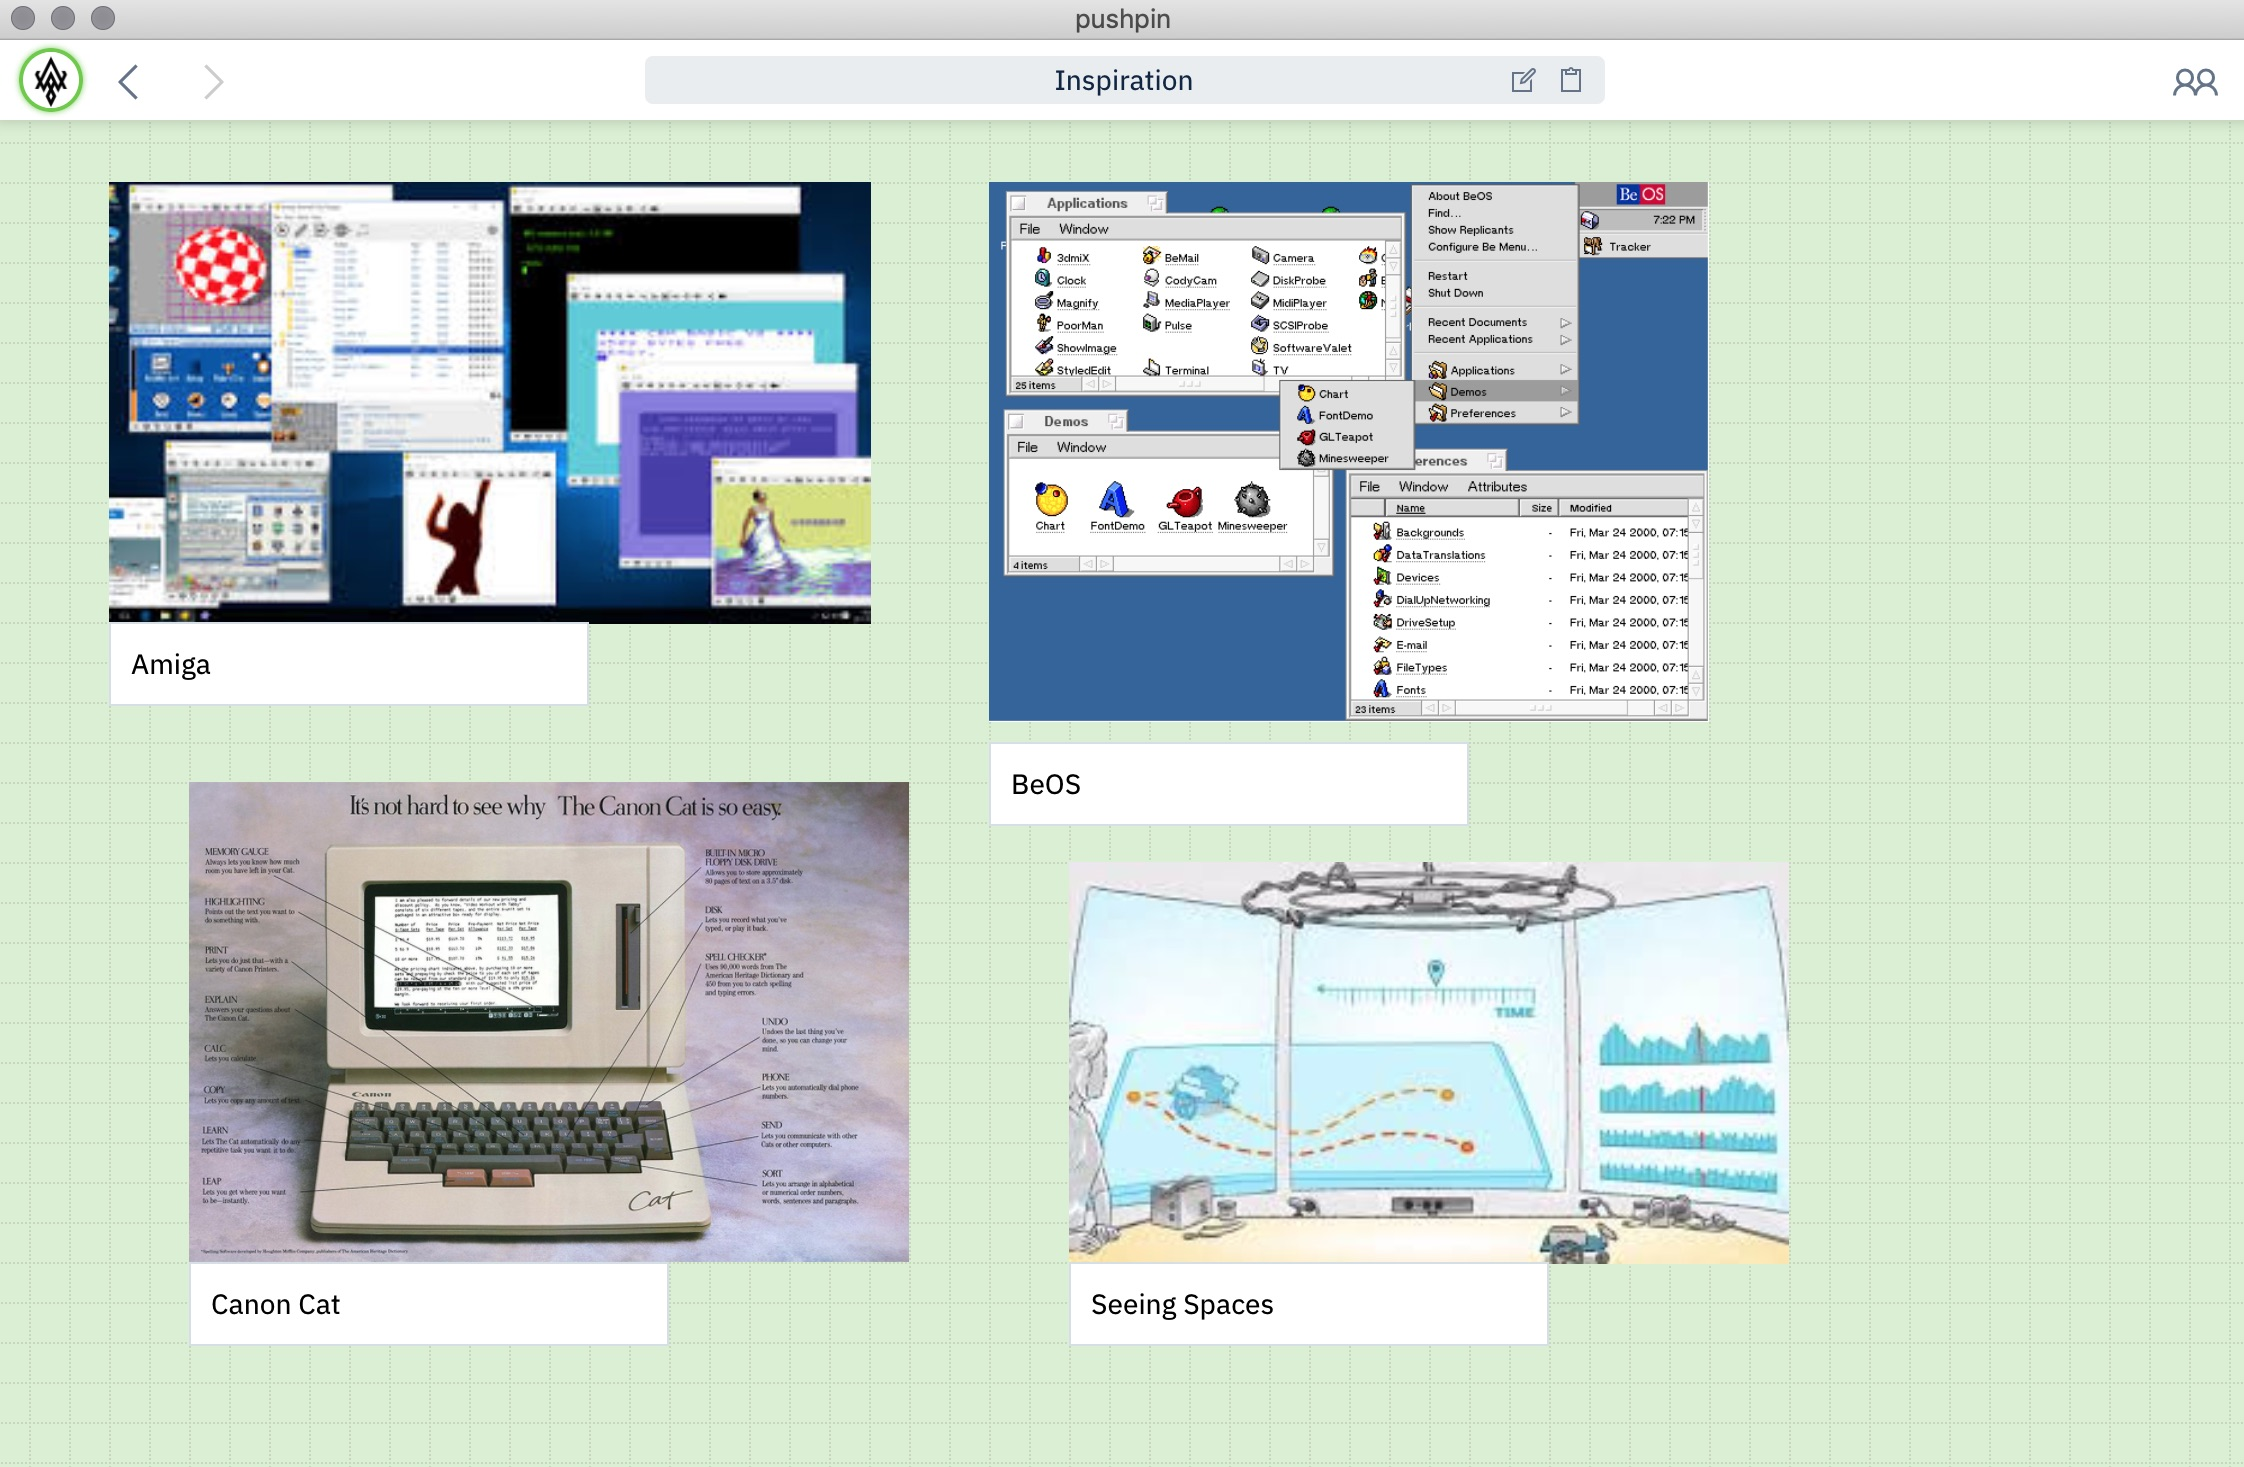
\includegraphics[width=0.7\textwidth]{pushpin.jpg}
    \caption{Screenshot of PushPin. The main user interface consists of cards of various types (text, image, PDF, \dots) that can be freely arranged on a 2D ``board''. Boards can be nested within other boards. The toolbar at the top provides navigation between boards and sharing settings.}
    \label{fig:pushpin}
\end{figure*}

\section{PushPin: A Collaborative Corkboard}

The PushPin software~\cite{PushPinSource}, shown in Figure~\ref{fig:pushpin}, allows users to collect media of various types (including text, web pages, images, and PDF files), to archive and organise it.
Media files are visually represented as \emph{cards} on an infinite 2D \emph{board}, where they can be resized and positioned arbitrarily.
One board may be nested within another board, enabling hierarchical organisation and navigation.
This board metaphor is known from other note-taking software such as Miro~\cite{Miro} and Milanote~\cite{Milanote}.

In recent years there has been considerable innovation in technologies for creating web applications, including in web browsers (new features of HTML and CSS), languages (e.g.\ TypeScript), user interface libraries (especially React~\cite{React}), and JavaScript modules for a wide variety of tasks (e.g.\ PDF rendering~\cite{PDFjs}).
In order to take advantage of this lively ecosystem, we decided to implement PushPin using web technologies.

However, web applications running in a browser tab have constraints that make them unsuitable for peer-to-peer use.
In particular, although web apps can write data to disk using APIs such as localStorage and IndexedDB, this data tends not to be very durable: it is silently deleted when a user chooses to clear cookies in their browser~\cite{LocalStorageCleared}.
(Maybe the clue is in the name: they are called ``browsers'', not ``keepers''.)

We avoid these limitations by building on Electron (TODO reference), which takes a JavaScript web app, runs it in a Chromium-based browser window, and allows the result to be packaged as a downloadable and locally installable executable.
Electron makes the full set of Node.js APIs available to application code, including full access to the local filesystem, and socket APIs allowing full TCP and UDP networking.
Electron apps are portable across Windows, Linux, and macOS.


\subsection{Network technologies}

% Many P2P protocols require sending and receiving arbitrary UDP packets.
% However, web browsers restrict network communication for security reasons, in particular through the \emph{same-origin policy}~\cite{SameOrigin}, making it impossible to implement such protocols in JavaScript alone.
% An exception is WebRTC, a P2P protocol that is built into web browsers.

% Designed to collect all the information you need and synchronize it across all your computers. PushPin supports taking notes, and can archive web content, images, PDFs, audio, video, and any other files you might want to hang out. It can synchronize across all your devices, and doesn't require any infrastructure to operate.


\subsection{Document-oriented Programming}
\begin{itemize}
    \item crdts
    \item frp
    \item peer-to-peer data distribution
\end{itemize}

\section{Bullet Points}

Before describing our solution, let us first outline the challenges of a decentralised application system.

\section{Challenges of Developing an Intrinsically Distributed System}

If we embrace both the notion that access to data from any computer is essential, and that mandatory centralised infrastructure is antithetical to the goal of permanently available software then it becomes inevitable that we must build a peer-to-peer data distribution system. 

Peer-to-peer systems have a number of unique challenges versus centralised systems, including:

\begin{itemize}
	\item no single source of truth, no single authority

	Without a centralised server hosting an authoritative copy, every copy of the data becomes, in some sense, authoritative. This implies that we must have some kind of robust merging strategy at the core of our design.
	\item devices get out of sync

    Because we insist that each device is always able to make progress without communication with other nodes, it is vitally important to both do our best to synchronise our various devices, but also to communicate synchronisation state. What were the last changes received from our laptop? Did the changes we made locally get uploaded to a server before the network connection was lost?  

    \item connectivity is non-boolean

    With a centralised system a user is either offline or online. The central node routes all data. With a peer-to-peer system is is entirely possible that you might be connected with another user around the world but due to the complexities of computer networking, disconnected from a user in the same room. (Perhaps their wifi connection is offline.) 

    \item changes can come from anywhere at any time

    Without the centralised system approving or rejecting changes against a monotonically incrementing API version, it's possible that other clients are running older, newer, or just different versions of the program. How do we robustly manage change over time?
\end{itemize}

\section{How to actually build within these constraints}

At first glance, these challenges may appear insurmountable. We want to store all the data a user is exposed to permanently on all their devices, to allow differing versions of the software to inter-operate, to enable collaboration between users in every possible combination of devices and network topologies, and most challenging of all, we want to do all of this in a way that makes it easy for anyone with industry-standard web development skills to successfully produce software!

In fact, we have made significant progress towards this end by productively combining a number of recent developments in software methodology in a form we have not yet seen elsewhere. We call this approach "document oriented programming".

\subsection{Functional Reactive Programming}
The first motivating insight is that functional reactive programming is a helpful abstraction. Functional reactive programming works by creating a single, functional loop where a program state is deterministically transformed into a user interface, and where all interactions emitting from the user interface pass through a single function (known as a reducer) which produce the next state.

In the simplest case, we tie the program state to an operational CRDT (automerge), and record all changes to that program state into a per-client append-only log which we can broadcast to our other peers. Visibility vectors preserve causality of changes, and for further details of how this process works, please see <some reference here>.

\begin{figure}
    \centering
    % diagram depicting FRP + CRDTs here
    %\includegraphics{}
    \caption{Caption}
    \label{fig:my_label}
\end{figure}

\subsection{Peer-to-peer Networking}

Distribution of local changes is managed via a peer-to-peer system akin to the Dat Project \ref{}. Append-only logs are identified by the public half of a key-pair, and changes are signed by the private half. This allows any participating peer to serve requests for data in a trustworthy fashion.  

Actually establishing peer-to-peer connections is challenging in real-world computer systems. Chief among problems is the tendency for user computers to be situated behind NAT firewalls. A variety of peer-discovery and NAT traversal methods are common-place in peer-to-peer systems, but we cannot take advantage of industry standards like uPNP (as the BitTorrent software often does) because we want our software to work successfully in environments where the user does not control network infrastructure like at cafe's, in libraries, and on institutional networks.

% I feel like there is a lot more to say about document URLs and sharing here.

\subsection{Local State and Ephemeral State}

Our earliest prototypes assumed users would have only a single "document" open at a time, and that these documents would be shared by their URLs. We also made no allowances for non-shared state. This model was very limiting, and over time we found we needed a number of additional concepts.

First, and quite simply, by explicitly separating application state into a local-only and shared-document we enabled our application developers to keep track of local-only state like drafts of messages in text-boxes.

Next, we added a messaging system to allow users to broadcast parts of this local state to their peers. We use this to communicate data which is valuable only in the moment and not worthy of recording, such as another users' current selection, or cursor position in a text field.

\subsection{Composite Views}

As we approached more sophisticated usage, we came across a simple idea that enabled us to preserve our abstraction while pursuing much more elaborate software. By allowing a pairing of a shareable CRDT document with an FRP renderer to be nested inside another such construct we can build up complex networks of documents each with their own collaborators.

For example, we can define a "container" which renders a list of documents stored as a CRDT of document URLs, and a user might synchronise the full list across all their own devices, but only share some of them with their other collaborators.
% this is kind of poorly worded but i need to run...

% i think this is now covered above but left this here for reference
\begin{comment}
    how to rationalize all this?
    \begin{itemize}
	    \item FRP, for its easily reasoned-about loop: 
	    \begin{itemize}
			 \item transform a document functionally into an application view
			 \item create events in the application that trigger state updates
			 \item record \& broadcast state updates to peers
		\end{itemize}
	    \item many nested \& linked documents, each with their own render function
	    \begin{itemize}
		    \item a text note, a chat window, a user profile, a canvas
		\end{itemize}
	    \item store all local changes in append-only logs, distribute those logs to other interested peers
	    \item use cryptographic functions to produce self-validating data
	\end{itemize}
\end{comment}


what works, what's not working so well?

\begin{itemize}
    \item FRP render loop works great -- taking a functional transform of a document state to application view means never worrying about where the update came from or how to render it
	\item storing \& distributing append-only logs is very simple and robust
    \item peer-to-peer networking is highly problematic
    \begin{itemize}
	    \item webrtc (not very good, requires centralized assets)
		\item DHTs (reliability, privacy)
		\item centralized services (fragility)
		\item router configuration issues
	\end{itemize}
	\item much performance work has been done
	\begin{itemize}
	    \item architect to separate render \& computation of CRDT operations
	\end{itemize}
	\item conflict resolution surprisingly unproblematic
	\item merge \& collaboration UX is largely unexplored (could show a pixelpusher slide \& briefly explain problems)
	\item what kind of identity, privacy, sharing features are important / feasible here?
	\item html is a pretty rough application development platform
	\item no real mobile support
	\begin{itemize}
	    \item what's the cross-platform story?
	\end{itemize}
\end{itemize}

\section{Conclusions}
\begin{itemize}
	\item frp + crdt = pretty good
\end{itemize}

\begin{acks}
Thank you to Roshan Choxi, Ignatius Gilfedder, Mark McGranaghan, Jeff Peterson, and Matt Tognetti, who contributed to the development of PushPin.
The project was produced under the auspices of the Ink \& Switch research lab (\url{https://www.inkandswitch.com/}).
Martin Kleppmann is supported by a Leverhulme Trust Early Career Fellowship and by the Isaac Newton Trust.
\end{acks}

\bibliographystyle{ACM-Reference-Format}
\bibliography{references}{}
\end{document}
